\section{Ruby On Rails}
I følgende afsnit, vil vi kort beskrive Ruby on Rails, som er et open-source framework til udvikling af web-applikationer, som vores system bygger på. Vi vil desuden forklarer Model-View-Controller arkitekturen, som er den arkitektur alle Ruby on Rails applikationer tager udgangspunkt i.  

Ruby on Rails (RoR) blev udviklet i 2003 af David Heinemeier Hansson(xxx KILDE xxx), og er et forholdsvist nyt web-applikationens framework, set i forhold til eksempelvis PHP, Java og .NET(xxx KILDE xxx). David Heinemeier Hanssons intentioner med RoR var, at skabe et framework, som gjorde det lettere og hurtigere for web-programmører at udvikle webapplikationer, hvilket også er en af de væsentlige åresager til at vi valgte at anvende det. Dette gjorde han bl.a. ved at implementere filosofien: {\emph{``konventioner over konfigurationer''}(xxx KILDE xxx) i RoR. Filosofien har både sine fordele og ulemper. Det er en ulempe, at web-udvikleren skal have arbejdet med RoR i lang tid, for at kunne huske de mange konventionerne; eller bruge en masse tid, på at slå dem op. Det er på den anden siden en fordel at web-udviklere, ved hjælp af RoR's konventioner, kan lave applikationer, som kan udrette meget, ud fra få linjer kode. RoR viser allerede fra første møde, når man genererer en ny web-applikation, at der skal meget lidt arbejde til, at få et stort afkast. Dette kan ses i billede \figref{fig:Rails-new-foodl}, hvor en enkelt linje i kommandopromten, generere en ny mappe, som indeholder en fuldtfungerende Ruby on Rails web-applikation, kaldet ``Foodl''. Mappen med web-applikationen består af en lang række undermapper. Heriblandt ``App'', hvori ``models'', ``views'' og ``controllers'' befinder sig; ``Config'', hvori ``routes'' befinder sig, som er det element der forbinder controllers og views (mere om dette i følgende sektion \cite{MVC}); og undermappen ``Spec'', hvori unit testing af Models, Views og Controllers foregår; samt flere. Kort sagt genererer rails, vha. new-kommandoen, hele skelettet for web-applikationen, og derefter er det ``bare'' at fylde det indhold man ønsker i sin web-applikation, i de rigtige mapper. Ønskes der yderligere information om Ruby on Rails, og sammenspillet mellem Rails og Ruby, henvises til \cite{RoR.org}.

\begin{figure}
\centering
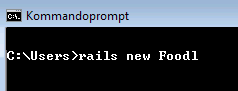
\includegraphics[scale=0.6]{billeder/Rails-new-foodl.png}
\capt{Railskommando, der indtastes i kommandopromten, hvorefter rails genererer en mappe med en fuldtfungerende web-applikation, kaldet ``Foodl''}
\label{fig:Rails-new-foodl}
\end{figure}

\subsection{Model-View-Controller}
\label{MVC}
Model-View-Controller (MVC) er den arkitektur en hver Ruby on Rails applikation tager udgangspunkt i. Så snart en ny Ruby on Rails web-applikation bliver genereret, vil den indeholder mapperne ``models'',``views'' og ``controllers'', så på den måde er en RoR applikation tvunget til at implementere MVC-arkitekturen. Arkitekturen blev opfundet af Trygve Reenskaug i 1979, som en slags standard arkitektur for interaktive applikationer (eksempelvis web-applikationer). Arkitekturen består af tre komponenter, nemlig modeller, views og controllers, der hverisær har nogle specifikke egenskaber og opgaver. Modellen den komponent, der har ansvaret for at applikationen 